\chapter{Experimental Setup}
\label{chapterlabel4}

Chapter~\ref{chapterlabel3} introduces the Dynamic Author-Topic model. In Chapter~\ref{chapterlabel4} we will introduce the design of the experiment related to our model. 



\section{Dataset}\label{dataset}
News is the contemporary witnesses of the world and tremendous number of news are generated every day. According to Chartbeat\footnote{http://www.slideshare.net/chartbeat/mockup-infographicv4-27900399}, over 92,000 news are posted to the web every 24 hours which is nearly impossible for human processing and tagging. Therefore BBC News Lab has launched the project \footnote{http://bbcnewslabs.co.uk/projects/topic-modeling/} collaborating with UCL to try to automatically nail down "What is this news about?" in a few words. 
The news stream is provided by BBC news using \textit{The Juicer} which is a news aggregation and content extraction API \footnote{http://bbcnewslabs.co.uk/projects/juicer/}. In order to capture the dynamic nature of the news we have crawed the BBC news in a long time range - from January 1st, 2016 to May 31st, 2016 - for the experiment's purpose.
The corpus has collected all 36,162 news published by BBC covering the period of 152 days. For the purpose of experimenting dynamic author-topic model we assume the news in a streaming scenario and are divided by a certain time interval. The news fall in the same time period are considered as exchangeable, with static nature. The time periods we set in the experiments are 7 days, 14 days, 28 days respectively. 

The news gathered from Jucier API is in the format of 
\begin{equation}\label{apiformat}
\{Subcategory, URL, News header, News body, Time\}
\end{equation}
and the news are falling into 106 subcategories which can be grouped into 9 categories as shown in Table~\ref{tab:news_category}, which you can always see on the BBC news website. 

Since we only need \textit{clean} news body for the model training purpose therefore the following pipeline shown in Figure~\ref{fig:pipeline} used to preprocess the news. The unnecessary tags, URL and timestamp in the raw data are removed firstly, followed by eliminating meaningless symbols. Then the stop words which are the most common words in a language are filtered out with all word tokens being downcased, and stemming is applied lastly to reduce inflectional forms and  derivationally related forms of a word to a common base form. Finally in total 29,448 unique word tokens are used for our model training.
\begin{figure}[h]
\centering
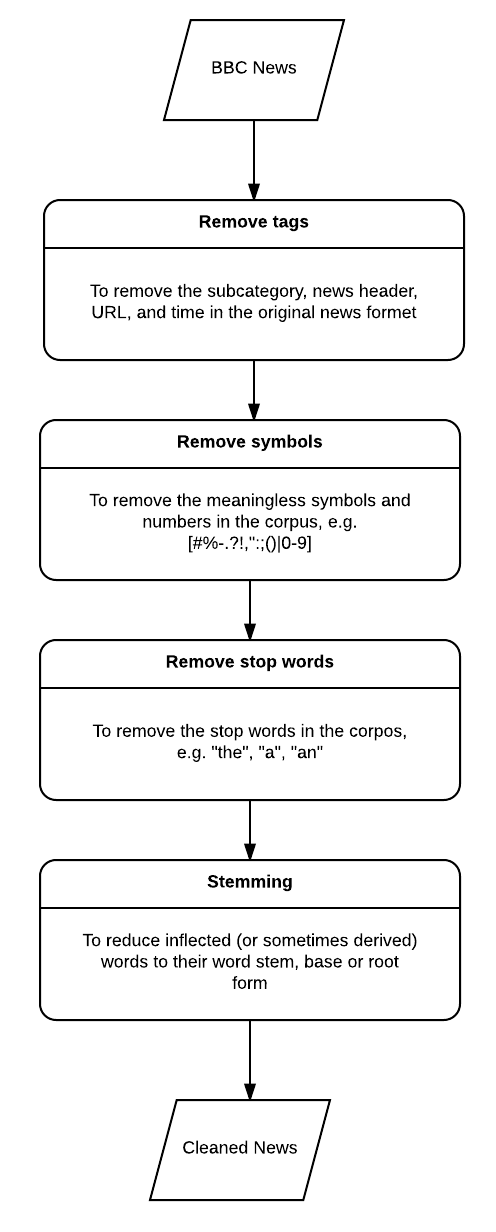
\includegraphics[width=0.5\textwidth]{figures/pipeline.png}
\caption{Preprocessing pipeline for BBC news}
\label{fig:pipeline}
\end{figure}

\begin{table}[h]
\centering
\begin{tabular}{l | p {10cm}}

Category & Subcategories examples\\
\hline 
1. UK & uk\_england;uk\_england\_essex;uk\_england\_nottingha\_shire;
uk\_scotland\_edinburgh\_east\_fife;uk\_wales\\
2. World & world\_asia\_china;world\_latin\_america;world\_us\_canada;
world\_radio\_and\_tv\\
3. Business & business\_your\_money;business \\
4. Politics & election\_england;election\_us \\
5. Tech & technology \\
6. Science & science\_environment\\
7. Heath & health  \\
8. Education & education \\
9. Entertainment \& Arts & entertainment\_arts \\
\hline
\end{tabular}
\caption{BBC news category and examples of subcategories}
\label{tab:news_category}
\end{table}

Statistically, we have calculated the \textit{word count} , indicating how many times a certain word token appears in the whole news corpus, and also \textit{file count}, indicating a certain word token has occurred in how many different news. 
Both of \textit{word count} and \textit{file count} follow the long tail distribution \cite{feldmann1997fitting}. Specifically, for \textit{word count}, 51\% of the total word tokens appears less than 20 times in the whole corpus, with the top 10 popular words as shown in Table~\ref{wordcount}.
\begin{table}[h!]
\centering
 \begin{tabular}{||c c||} 
 \hline
 Word & Word Count Occurrence \\ [0.5ex] 
 \hline\hline
  police	& 22587 \\
govern	& 	19257\\
work	& 	18185\\
could	& 	15619\\
uk	& 	15386\\
report		& 14995\\
first	& 	14555\\
told	& 	14213\\
bbc		& 14046\\
make	& 	13445 \\ [1ex] 
 \hline
 \end{tabular}
 \caption{Word count distribution: top 10 popular ones}
 \label{wordcount}
\end{table}

While for \textit{file count}, 60\% of the total word token appears in less than 20 different news. The top 10 popular words as shown in Table~\ref{filecount}.

\begin{table}[h!]
\centering
 \begin{tabular}{||c c||} 
 \hline
 Word & File Count Occurrence \\ [0.5ex] 
 \hline\hline
work &	9741 \\
could &		9341\\
first &		8835\\
take &		8675\\
told &		8669\\
police	 &	8576\\
include	 &	8479\\
make &		8475\\
bbc	 &	8395\\
report	 &	8192\\ [1ex] 
 \hline
 \end{tabular}
 \caption{File count distribution: top 10 popular ones}
 \label{filecount}
\end{table}


\section{Baselines}
We have compared our DAT model with a number of baselines which are classical algorithms. 
\begin{itemize}
    \item \textbf{Latent Dirichlet Allocation Model}: The temporal factor is not taken into consideration when classifying the news corpus as well as the author information. Related works are discussed in Section~\ref{lda} and mathematical details for experiments are presented in \ref{4lda}.
     \item \textbf{Author Topic Model}: This is a hierarchical generative model where each word
$w$ in a news is associated with two latent variables author $x$ and topic $z$. Temporal factor is not considered here. Related works are discussed in Section~\ref{2at} and experimental setups are shown in \ref{Author-Topic model}.
      \item \textbf{Topic Tracking Model}: This is a type of dynamic topic model with considering the dependency between news in the stream. We have discussed the related literature in Section~\ref{2tot} and how we experiment on this model in \ref{4tot}. 
\end{itemize}

In Section \ref{4lda},~\ref{Author-Topic model} and~\ref{4tot}, we will briefly introduce the three baseline models in terms of model description and experimental setups. The notations we used here can be referred in Table~\ref{tab:notation-des}.
\subsection{Latent Dirichlet Allocation Model}\label{4lda}

LDA model can be viewed as a generative model, which can be described as follows,
\begin{enumerate}
   \item For each topic $k \in [1,K]$
   \begin{enumerate}
     \item Draw a multinomial $\vec{\phi_k}$ from a Dirichlet prior $\vec{\beta}$
    \end{enumerate}
    \item For each news $m \in [1,M]$
     \begin{enumerate}
     \item Draw a multinomial $\vec{\theta}_m}}$ from a Dirichlet prior $\vec{\alpha}$
     
     \item For each word $n \in [1,N_m]$ in document $m$
     \begin{enumerate}
            \item Draw a topic assignment $z_{m,n}$ from per-author multinomila distribution over topic $\vec{\theta}_{m}$ %$\vec{\theta_{x_{m,n}}}$
            \item Draw a word $w_{m,n}$ from multinomial $\vec{\phi}_{z_{m, n}}$
            %$\vec{\phi_{z_{m,n}}}$
    \end{enumerate}
    \end{enumerate}
        
\end{enumerate}

Therefore the posterior distribution of the topics depends on the information from the news corpus. The parameterization of the LDA model is as follows,

\begin{eqnarray*} \label{eq:lda}
\boldsymbol{\Theta}_m | \boldsymbol{\alpha} & \sim & \text{Dirichlet}(\boldsymbol{\alpha})\\
\boldsymbol{\Phi_{k}} | \boldsymbol{\beta} & \sim & \text{Dirichlet}(\boldsymbol{\beta})\\
z_{m,n} | \boldsymbol{\Theta_{m}} & \sim & \text{Multinomial}(\boldsymbol{\Theta_{m}})\\
w_{m,n} | \boldsymbol{\Phi_{z_{m,n}}} & \sim & \text{Multinomial}(\boldsymbol{\Phi_{z_{m,n}}})\\

\end{eqnarray*}
with its graphical model representation in Figure~\ref{fig:lda}.

\begin{figure}[h]
\centering
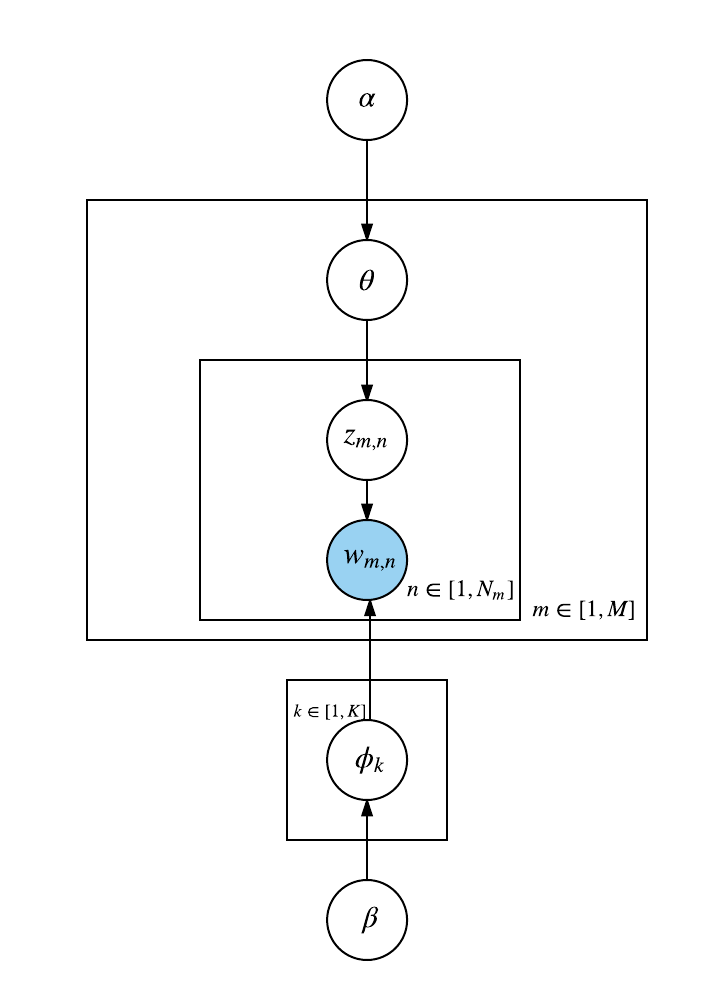
\includegraphics[width=0.6\textwidth]{figures/LDA.png}
\caption{Graphical representation of LDA topic model}
\label{fig:lda}
\end{figure}

As discussed in \cite{newman2007distributed} the exact inference of LDA model is intractable, we can only employ the Gibbs sampling method as an approximate method \cite{griffiths2002gibbs}. Finally we can implement our experiments based on the way to calculate the conditional probability of the topic in~\ref{\label{lda_z} to update the topics for each work token in each iteration. 

\begin{align}\label{lda_z}
\multicolumn{2} =   &  \math{P}({z}_{m, n}| \mathbf{w},\mathbf{z}_{\neg(m, n)},\alpha, \beta)  \nonumber
\displaybreak[3]\\ \nonumber
= & \quad \frac{\math{P}({w}_{m, n},{z}_{m, n}| \mathbf{w}_{\neg(m, n)},\mathbf{z}_{\neg(m, n)},\mathbf{x}, \alpha, \beta)}{\math{P}({w}_{m, n}| \mathbf{w}_{\neg(m, n)},\mathbf{z}_{\neg(m, n)},\mathbf{x}, \alpha, \beta)}
\displaybreak[3]\\ \nonumber
= & \quad \frac{P(\mathbf{w}, \mathbf{z} | \mathbf{x}, \alpha, \beta)}{P(\mathbf{w}, \mathbf{z}_{\neg(m,n)} |\mathbf{x}, \alpha, \beta)} \displaybreak[3]\\ \nonumber
= & \quad \frac{P(\mathbf{w}, \mathbf{z} | \mathbf{x}, \alpha, \beta)}{P(\mathbf{w}_{t,\neg(m,n)}, \mathbf{z}_{t,\neg(m,n)} | \mathbf{x},\alpha, \beta)P(w_{m,n} | \mathbf{x}, \alpha, \beta)} \displaybreak[3]\\ \nonumber
\propto & \quad \frac{P(\mathbf{w}, \mathbf{z} | \mathbf{x}, \alpha, \beta)}{P(\mathbf{w}_{\neg(m,n)}, \mathbf{z}_{\neg(m,n)} | \mathbf{x},\alpha, \beta)} \displaybreak[3]\\ \nonumber 
\propto & \quad  \left(\frac{n_{v,k}+\beta_{k,v}-1}{\sum_{v=1}^V \left(n_{v,k}+\beta_{v,k} \right)-1 } \right) \times   \left(\frac{n_{a,k}+\alpha_{k} -1}{\sum_{k=1}^K \left(n_{a,k}+\alpha_{k} \right)-1 } \right).
\displaybreak[3]\\
\end{align}

The parameter sets $\boldsymbol{\Theta}$ and $\boldsymbol{\Phi}$ can be obtained with \eqref{lda_phi} and \eqref{lda_theta}.

\begin{equation}\label{lda_phi}
\phi_{k,v} = \frac{n_{k,v} + \beta_{v}}{\sum_{v=1}^V(n_{k,v} + \beta_v)}.
\end{equation}

\begin{equation}\label{lda_theta}
\theta_{m,k} = \frac{n_{m,k} + \alpha_{k}}{\sum_{k=1}^K(n_{m,k} + \alpha_k)}.
\end{equation}

The Gibbs sampling algorithm runs over the three periods of initialization, burn-in and sampling. The algorithm procedures that we have employed for our experiments is shown as Algorithm 2.
\begin{algorithm}\label{algo:lda}
\DontPrintSemicolon
\LinesNotNumbered
 
    \SetKwInOut{Input}{Input}
    \SetKwInOut{Output}{Output}
    \SetKwInOut{Parameter}{Global Data}

    \Input{word vector $\boldsymbol{w}$, $\alpha$,$\beta$, topic number $K$}
    \Parameter{count statistics $\{n_{m,k}\}$, $\{n_{k,v}\}$, and their sums $\{n_{m}\}$, $\{n_{k}\}$}
    \Output{topic associations $\boldsymbol{z}$, multinomila parameter $\boldsymbol{\Phi}$, and $\boldsymbol{\Theta}$}
    {// \textbf{Initialization}:}\;
    zero all count variables: $\{n_{m,k}\}$, $\{n_{k,v}\}$, $\{n_{m}\}$, $\{n_{k}\}$\;
    
    \For{all news $m \in [1,M]$ }{
      \For{all words $n \in [1,N_m]$ in news m }{
      sample topic index $z_{m,n} = k \sim \text{Multinomial}(1/K)$ \par
      increment author-topic count: $n_{m,k} += 1$\par
      increment author-topic sum: $n_{m} += 1$\par
      increment topic-word count: $n_{k,w_{m,n}} += 1$\par
      increment topic-word count: $n_{k} += 1$\par
      }
   }
   {// \textbf{Gibbs Sampling}:}\;
    sample over burn-in period and sampling period:\; 
    \caption{Inference for the LDA model using Gibbs sampling }
    \While{not finished}{
    \For{all news $m \in [1,M]$ }{
      \For{all words $n \in [1,N_m]$ in news m }{
      // For the current assignment of $k$ to the word token $w_{m,n}$ \par
      decrement author-topic count: $n_{m,k} -= 1$\par
      decrement author-topic sum: $n_{m} -= 1$\par
      decrement topic-word count: $n_{k,w_{m,n}} -= 1$\par
      decrement topic-word count: $n_{k} -= 1$\par
      sample topic index $\boldsymbol{z} \sim P(z_{m,n}|\boldsymbol{x},\boldsymbol{z}_{(\neg{m,n})},\boldsymbol{w},\boldsymbol{\alpha},\boldsymbol{\beta})$ according to~\eqref{lda_z}\par
      // For the new assignment of $k$ to the word token $w_{m,n}$ \par
      increment author-topic count: $n_{m,k} += 1$\par
      increment author-topic sum: $n_{m} += 1$\par
      increment topic-word count: $n_{k,w_{m,n}} += 1$\par
      increment topic-word count: $n_{k} += 1$\par
      
      }
   }
    }
    \If{converged}{
    read out parameter set $\boldsymbol{\Phi}$ according to~\eqref{lda_phi}\par
    read out parameter set $\boldsymbol{\Theta}$ according to~\eqref{lda_theta}\par
    }

\end{algorithm}


\subsection{Author-Topic Model} \label{Author-Topic model}

Author Topic model can be viewed as a hierarchical generative model, which can be described as follows,
\begin{enumerate}
   \item For each topic $k \in [1,K]$
   \begin{enumerate}
     \item Draw a multinomial $\vec{\phi_k}$ from a Dirichlet prior $\vec{\beta}$
    \end{enumerate}
   \item For each author $a \in [1,A]$
   \begin{enumerate}
     \item Draw a multinomial $\vec{\theta_a}$ from a Dirichlet prior $\vec{\alpha}$
    \end{enumerate}
    \item For each news $m \in [1,M]$
   \begin{enumerate}
     \item For each word $n \in [1,N_m]$ in document $m$
     \begin{enumerate}
            \item Draw an author $x_{m,n}$ uniformly from the group of authors $a_M$
            \item Draw a topic assignment $z_{m,n}$ from per-author multinomila distribution over topic $\vec{\theta}_{x_{m, n}}$ %$\vec{\theta_{x_{m,n}}}$
            \item Draw a word $w_{m,n}$ from multinomial $\vec{\phi}_{z_{m, n}}$
            %$\vec{\phi_{z_{m,n}}}$
    \end{enumerate}
    \end{enumerate}
        
\end{enumerate}

The posterior distribution of topics depends on the information from the news corpus and also the authors set, the parameterization of the Author-Topic model is 
\begin{eqnarray*} \label{eq:at}
\boldsymbol{\Theta}_a | \boldsymbol{\alpha} & \sim & \text{Dirichlet}(\boldsymbol{\alpha})\\
\boldsymbol{\Phi_{k}} | \boldsymbol{\beta} & \sim & \text{Dirichlet}(\boldsymbol{\beta})\\
z_{m,n} | \boldsymbol{\Theta_{x_{m,n}}} & \sim & \text{Multinomial}(\boldsymbol{\Theta_{x_{m,n}}})\\
w_{m,n} | \boldsymbol{\Phi_{z_{m,n}}} & \sim & \text{Multinomial}(\boldsymbol{\Phi_{z_{m,n}}})\\
x_{m,n} | A_m & \sim & \text{Multinomial}(1/A_m)\\

\end{eqnarray*}

Using the graphical model, the AT model can be shown as in Figure~\ref{fig:at}. The inference of the model is done by Gibbs sampling.As dicussed in \cite{rosen2010learning}, the conditional probability of the topic and author for sampling in each iteration is shown in~\eqref{at_x} and~\eqref{at_z}.
\begin{figure}[h]
\centering
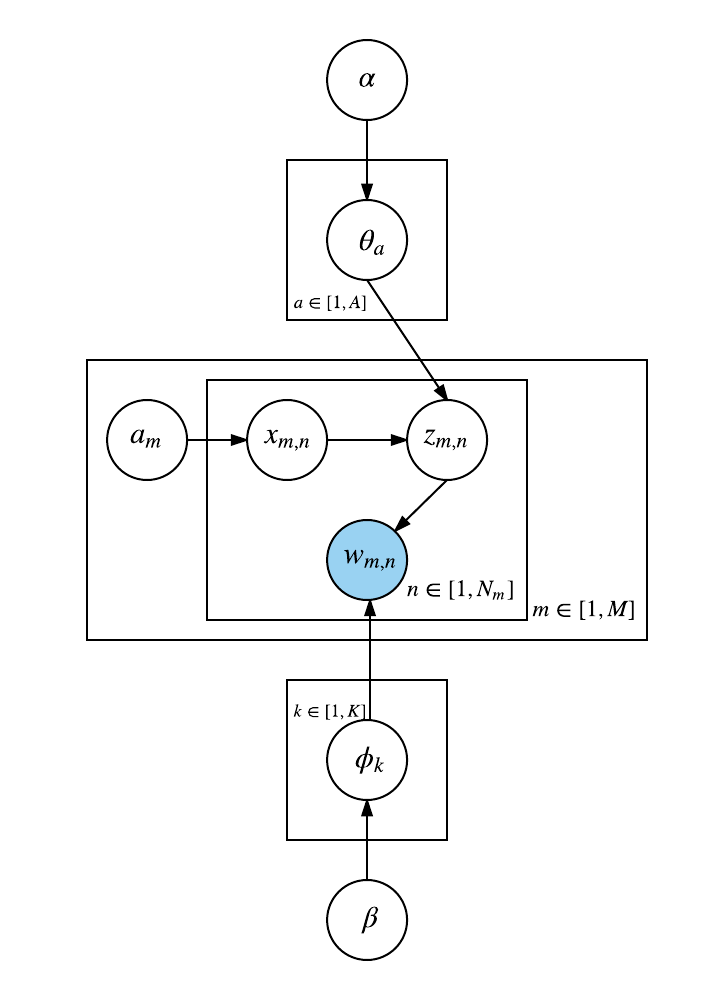
\includegraphics[width=0.6\textwidth]{figures/AT.png}
\caption{Graphical representation of Author-Topic model}
\label{fig:at}
\end{figure}

\begin{align}\label{at_z}
\multicolumn{2} =   &  \math{P}({z}_{m, n}| \mathbf{w},\mathbf{z}_{\neg(m, n)},\mathbf{x},\alpha, \beta)  \nonumber
\displaybreak[3]\\ \nonumber
= & \quad \frac{\math{P}({w}_{m, n},{z}_{m, n}| \mathbf{w}_{\neg(m, n)},\mathbf{z}_{\neg(m, n)},\mathbf{x}, \alpha, \beta)}{\math{P}({w}_{m, n}| \mathbf{w}_{\neg(m, n)},\mathbf{z}_{\neg(m, n)},\mathbf{x}, \alpha, \beta)}
\displaybreak[3]\\ \nonumber
= & \quad \frac{P(\mathbf{w}, \mathbf{z} | \mathbf{x}, \alpha, \beta)}{P(\mathbf{w}, \mathbf{z}_{\neg(m,n)} |\mathbf{x}, \alpha, \beta)} \displaybreak[3]\\ \nonumber
= & \quad \frac{P(\mathbf{w}, \mathbf{z} | \mathbf{x}, \alpha, \beta)}{P(\mathbf{w}_{t,\neg(m,n)}, \mathbf{z}_{t,\neg(m,n)} | \mathbf{x},\alpha, \beta)P(w_{m,n} | \mathbf{x}, \alpha, \beta)} \displaybreak[3]\\ \nonumber
\propto & \quad \frac{P(\mathbf{w}, \mathbf{z} | \mathbf{x}, \alpha, \beta)}{P(\mathbf{w}_{\neg(m,n)}, \mathbf{z}_{\neg(m,n)} | \mathbf{x},\alpha, \beta)} \displaybreak[3]\\ \nonumber 
\propto & \quad  \left(\frac{n_{v,k}+\beta_{k,v}-1}{\sum_{v=1}^V \left(n_{v,k}+\beta_{v,k} \right)-1 } \right) \times   \left(\frac{n_{a,k}+\alpha_{k} -1}{\sum_{k=1}^K \left(n_{a,k}+\alpha_{k} \right)-1 } \right).
\displaybreak[3]\\
\end{align}
 
\begin{align}\label{at_x}
\multicolumn{2} =   &  \math{P}({x}_{m, n}| \mathbf{z},\mathbf{x}_{\neg(m, n)}, \mathbf{a},\alpha) \nonumber
\displaybreak[3]\\ \nonumber
= & \quad \frac{\math{P}({x}_{m, n},{z}_{m, n}| \mathbf{x}_{\neg(m, n)},\mathbf{z}_{\neg(m, n)}, \mathbf{a},\alpha)}{\math{P}({z}_{m, n}| \mathbf{x}_{\neg(m, n)},\mathbf{z}_{\neg(m, n)}, \mathbf{a},\alpha)}
\displaybreak[3]\\ \nonumber
= & \quad \frac{P(\mathbf{x}, \mathbf{z} | \mathbf{a}, \alpha)}{P(\mathbf{z}, \mathbf{x}_{\neg(m,n)} | \mathbf{a},\alpha)} \displaybreak[3]\\ \nonumber
= & \quad \frac{P(\mathbf{x}, \mathbf{z} | \mathbf{a}, \alpha)}{P(\mathbf{x}_{\neg(m,n)}, \mathbf{z}_{\neg(m,n)} | \alpha, \mathbf{a})P(z_{m,n} |  \alpha, \mathbf{a})} \displaybreak[3]\\ \nonumber
= & \quad \frac{P(\mathbf{x}, \mathbf{z} | \mathbf{a}, \alpha)}{P(\mathbf{x}_{\neg(m,n)}, \mathbf{z}_{\neg(m,n)} | \alpha, \mathbf{a})} \displaybreak[3]\\ \nonumber
%
\propto & \quad   \left(\frac{n_{a,k}+\alpha_{k} -1}{\sum_{k=1}^K \left(n_{a,k}+\alpha_{k} \right)-1 } \right).
\displaybreak[3]\\
\end{align}

By calculating the expectation of the Dirichlet distribution of $\boldsymbol{\Theta}$ and $\boldsymbol{\Phi}$ we can obtain the update rule as in~\eqref{at_phi} and~\eqref{at_theta}:


\begin{equation}\label{at_phi}
\phi_{k,v} = \frac{n_{k,v} + \beta_{v}}{\sum_{v=1}^V(n_{k,v} + \beta_v)}.
\end{equation}

\begin{equation}\label{at_theta}
\theta_{a,k} = \frac{n_{a,k} + \alpha_{k}}{\sum_{k=1}^K(n_{a,k} + \alpha_k)}.
\end{equation}

In Algorithm 3 we show how we employ our inference algorithm for Author-Topic model for the experiments. 


\begin{algorithm}\label{algo:AT}
\DontPrintSemicolon
\LinesNotNumbered
 
    \SetKwInOut{Input}{Input}
    \SetKwInOut{Output}{Output}
    \SetKwInOut{Parameter}{Global Data}

    \Input{word vector $\boldsymbol{w}$, author vector $\boldsymbol{a}$, $\alpha$,$\beta$, topic number $K$}
    \Parameter{count statistics $\{n_{a,k}\}$, $\{n_{k,v}\}$, and their sums $\{n_{a}\}$, $\{n_{k}\}$}
    \Output{topic associations $\boldsymbol{z}$, author associations $\boldsymbol{a}$, multinomila parameter $\boldsymbol{\Phi}$, and $\boldsymbol{\Theta}$}
    {// \textbf{Initialization}:}\;
    zero all count variables: $\{n_{a,k}\}$, $\{n_{k,v}\}$, $\{n_{a}\}$, $\{n_{k}\}$\;
    
    \For{all news $m \in [1,M]$ }{
      \For{all words $n \in [1,N_m]$ in news m }{
      sample topic index $z_{m,n} = k \sim \text{Multinomial}(1/K)$ \par
      sample author index $x_{m,n} = a \sim \text{Multinomial}(1/A_m)$ \par
      increment author-topic count: $n_{a,k} += 1$\par
      increment author-topic sum: $n_{a} += 1$\par
      increment topic-word count: $n_{k,w_{m,n}} += 1$\par
      increment topic-word count: $n_{k} += 1$\par
      }
   }
   {// \textbf{Gibbs Sampling}:}\;
    sample over burn-in period and sampling period:\; 
    \caption{Inference for the Author-Topic model using Gibbs sampling }
    \While{not finished}{
    \For{all news $m \in [1,M]$ }{
      \For{all words $n \in [1,N_m]$ in news m }{
      // For the current assignment of $k$ and $a$ to the word token $w_{m,n}$ \par
      decrement author-topic count: $n_{a,k} -= 1$\par
      decrement author-topic sum: $n_{a} -= 1$\par
      decrement topic-word count: $n_{k,w_{m,n}} -= 1$\par
      decrement topic-word count: $n_{k} -= 1$\par
      sample author index $\boldsymbol{a} \sim P(x_{m,n}|\boldsymbol{x}_{(\neg{m,n})},\boldsymbol{z},\boldsymbol{a},\boldsymbol{\alpha})$ according to~\eqref{at_x} \par
      sample topic index $\boldsymbol{z} \sim P(z_{m,n}|\boldsymbol{x},\boldsymbol{z}_{(\neg{m,n})},\boldsymbol{w},\boldsymbol{\alpha},\boldsymbol{\beta})$ according to~\eqref{at_z}\par
      // For the new assignment of $k$ and $a$ to the word token $w_{m,n}$ \par
      increment author-topic count: $n_{a,k} += 1$\par
      increment author-topic sum: $n_{a} += 1$\par
      increment topic-word count: $n_{k,w_{m,n}} += 1$\par
      increment topic-word count: $n_{k} += 1$\par
      
      }
   }
    }
    \If{converged}{
    read out parameter set $\boldsymbol{\Phi}$ according to~\eqref{at_phi}\par
    read out parameter set $\boldsymbol{\Theta}$ according to~\eqref{at_theta}\par
    }

\end{algorithm}


 
 
\subsection{Topic Tracking Model}\label{4tot}

The Topic Tracking model that we employed are based on the algorithms in \cite{liangdynamic} and \cite{iwata2009topic}. The difference of the TTM model with LDA and AT model is that the news is regarded as a stream and time is taken into consideration. The generative model of TTM at time $t$ is,

\begin{enumerate}
   \item For each topic $k \in [1,K]$
   \begin{enumerate}
     \item Draw a multinomial $\vec{\phi}_{t,k}$ from a Dirichlet prior $\vec{\beta}_{t,k}\vec{\phi}_{t-1,k}$
    \end{enumerate}
    \item For each news $m \in [1,M]$
   \begin{enumerate}
   \item Draw a multinomial $\vec{\theta}_{t,m}$ from a Dirichlet prior $\vec{\alpha}_t}}\vec{\theta}_{t-1}$
     \item For each word $n \in [1,N_m]$ in document $m$
     \begin{enumerate}
            \item Draw a topic assignment $z_{m,n}$ from per-author multinomila distribution over topic $\vec{\theta}_{m,t}$ %$\vec{\theta_{x_{m,n},t}}$
            \item Draw a word $w_{m,n}$ from multinomial $\vec{\phi}_{z_{m, n},t}$
            %$\vec{\phi_{z_{m,n},t}}$
    \end{enumerate}
    \end{enumerate}
        
\end{enumerate}

The parameterization of the TTM model is as follows,
\begin{eqnarray*} \label{eq:dat}
\boldsymbol{\Theta}_{t} | \boldsymbol{\alpha_{t}}
\boldsymbol{\Theta}_{t-1}
& \sim & \text{Dirichlet}({\boldsymbol{\alpha_{a,t}}
\boldsymbol{\Theta}_{a,t-1}})\\
\boldsymbol{\Phi_{k,t}} | \boldsymbol{\beta_{k,t}}\boldsymbol{\Phi_{k,t-1}} & \sim & \text{Dirichlet}(\boldsymbol{\beta_{k,t}}\boldsymbol{\Phi_{k,t-1}})\\
z_{m,n} | \boldsymbol{\Theta_{t}} & \sim & \text{Multinomial}(\boldsymbol{\Theta_{t}})\\
w_{m,n} | \boldsymbol{\Phi_{z_{m,n},t}} & \sim & \text{Multinomial}(\boldsymbol{\Phi_{z_{m,n},t}})\\
\end{eqnarray*}
and the graphical model representation of TTM is in Figure~\ref{fig:tot}.

\begin{figure}[h]
\centering
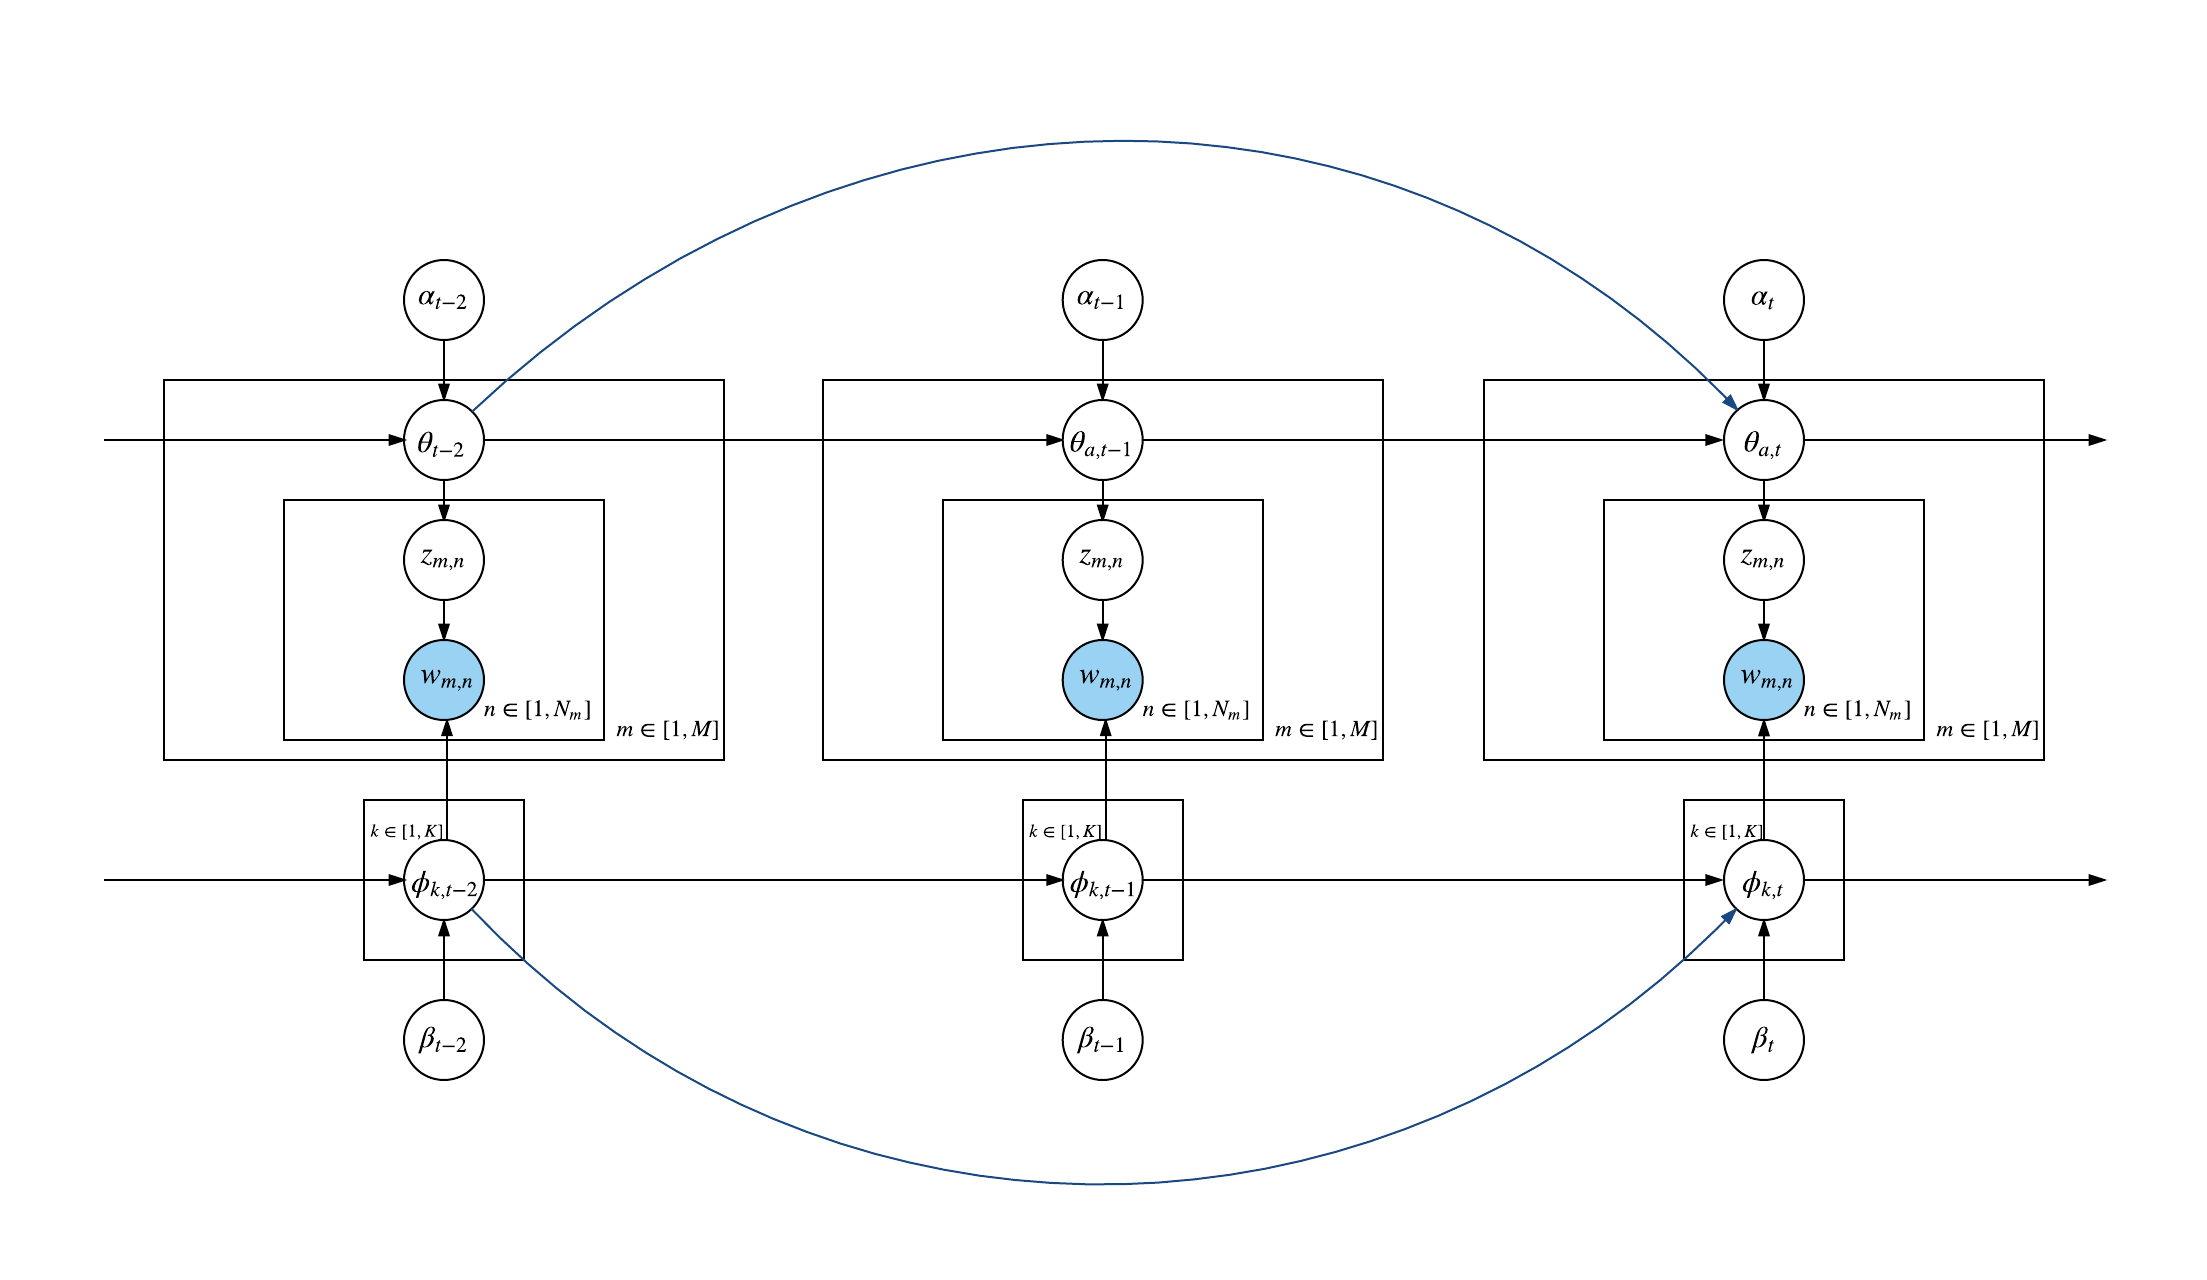
\includegraphics[width=\textwidth]{figures/TOT.png}
\caption{Graphical representation of Topic Tracking Model}
\label{fig:tot}
\end{figure}

Similar to the inference of LDA model, the assignment of the latent topic at time $t$ can be estimated using~\eqref{ttm_z},
\begin{align}\label{ttm_z}
\multicolumn{2} =   &  \math{P}({z}_{m, n, t}| \mathbf{w}_t,\mathbf{z}_{\neg(m, n, t)}, \alpha_t, \beta_t,\boldsymbol{\Phi}_{t-1}, \boldsymbol{\Theta}_{t-1}) \nonumber
\displaybreak[3]\\ \nonumber
\propto & \quad  \left(\frac{n_{t,v,k}+\beta_{t,k,v}\phi_{t-1}-1}{\sum_{v=1}^V \left(n_{t,v,k}+\beta_{t,v,k}\phi_{t-1} \right)-1 } \right) \times   \left(\frac{n_{t,m,k}+\alpha_{t,k} \Theta_{t-1}-1}{\sum_{k=1}^K \left(n_{t,m,k}+\alpha_{t,k}\theta_{t-1} \right)-1 } \right).
\displaybreak[3]\\
\end{align}
And by maximizing the joint distribution of topic $\boldsymbol{z}$ and word $\boldsymbol{w}$ as discussed in \cite{minka2000estimating}, we are able to obtain the update rules for the prevision values $\boldsymbol{\alpha}$ and $\boldsymbol{\beta}$ as shown in~\eqref{tot_alpha} and~\eqref{tot_beta},

\begin{equation}\label{tot_alpha}
\alpha_{t, k} \leftarrow \frac{\alpha_{t, k} \left( \Psi(m_{t, k} + \alpha_{t,k} \theta_{t-1, k}) - \Psi(\alpha_{t, k} \theta_{t-1, k}) \right)}{ \Psi(\sum_{k=1}^K m_{t, k} + \alpha_{t, z} \theta_{t-1, k}) - \Psi(\sum_{k=1}^Z \alpha_{t, k} \theta_{t-1, k}) },
\end{equation}
%
where $\Psi(\cdot)$ defined by $\Psi(x)=\frac{\partial\log\Gamma(x)}{\partial x}$ is the digamma function; whereas the following update rule of $\beta_t$ is,
%
\begin{equation}\label{tot_beta}
\beta_{t, k, v} \leftarrow  \frac{\sum_{k=1}^K \beta_{t, k, v} \phi_{t-1, k, v} \Psi(n_{t, k, v} +\beta_{t, k, v} \phi_{t-1, k, v}) - \Psi(\beta_{t, k, v} \phi_{t-1, k, v})}{ \sum_{k=1}^K \phi_{t-1, k, v}  \Psi(\sum_{v=1}^V n_{t, k, v} + \beta_{t, k, v} \phi_{t-1, k, v}) - \Psi(\sum_{v=1}^V \beta_{t, k, v} \phi_{t-1, k, v})}.
\end{equation}

After the iteration, the dynamic topic distribution at time $t$ can be inferred as \eqref{eq:thetatz} and \eqref{eq:phitzv},
\begin{align}
\label{eq:thetatz}
\theta_{t, k}  = & \frac{ m_{t, k} + \alpha_{t, k}\theta_{t-1, k} }{ \sum_{k=1}^K m_{t, k} + \alpha_{t, k} \theta_{t-1, k}} = \frac{ m_{t, k} + \alpha_{t, k}\theta_{t-1, k} }{ m_t + \sum_{k=1}^K \alpha_{t, k}\theta_{t-1, k} },
%=& \frac{ m_{t, z} + \alpha_{t, z}\theta_{t-1, z} }{ m_t + \sum_z \alpha_{t, z}\theta_{t-1, z} }
\end{align}
where $m_t$ is the total number of documents in $\mathbf{d}_t$, and infer a multinomial distribution over words for topic $z$ at time $t$ as,
%
\begin{equation}
\label{eq:phitzv}
%\phi_{t, z, v} =  \frac{ n_{t, z,v } + \beta_{t, z, v} \phi_{t-1, z, v} }{ \sum_v n_{t, z, v} + \beta_{t, z, v} \phi_{t-1, z, v} } =  \frac{ n_{t, z,v } + \beta_{t, z, v} \phi_{t-1, z, v} }{ n_{t,z} + \sum_v \beta_{t, z, v} \phi_{t-1, z, v} },
\phi_{t, k, v} =  \frac{ n_{t, k,v } + \beta_{t, k, v} \phi_{t-1, k, v} }{ n_{t,k} + \sum_{v=1}^V \beta_{t, k, v} \phi_{t-1, k, v} },
%=& \frac{ n_{t, z,v } + \beta_{t, z, v} \phi_{t-1, z, v} }{ n_{t,z} + \sum_v \beta_{t, z, v} \phi_{t-1, z, v} }
\end{equation}
where $m_{t,k}$ is the number of words assigned to news $m$ at time t, $n_{t, k}$ is the number of words assigned to topic $l$ at time $t$. Whereas $m_t$ is the sum-up of $m_{t,k}$ over all topics and $n_{t, k}$ is the sum-up of $n_{t, k, v}$ over all word tokens in the news corpus. In Algorithm 4 we will show how we employ this model for our experiment.
\begin{algorithm}\label{algo:TOT}
\DontPrintSemicolon
\LinesNotNumbered
 
    \SetKwInOut{Input}{Input}
    \SetKwInOut{Output}{Output}
    \SetKwInOut{Parameter}{Global Data}

    \Input{word vector $\boldsymbol{w}$, $\alpha$,$\beta$, topic number $K$}
    \Parameter{count statistics $\{n_{m,k}\}$, $\{n_{k,v}\}$, and their sums $\{n_{m}\}$, $\{n_{k}\}$}
    \Output{topic associations $\boldsymbol{z}$, multinomila parameter $\boldsymbol{\Phi}$, and $\boldsymbol{\Theta}$}
    \If{$t=0$}{
    Set initial values for $\boldsymbol{\Theta}$ as $1/K$ and $\boldsymbol{\Phi}$ as $1/V$, also for $\boldsymbol{\alpha}$ and $\boldsymbol{\beta}$  
    }
    \For{time $t \in [1,T]$}{
    {//  
    \textbf{Initialization}:}\;
    zero all count variables: $\{n_{m,k}\}$, $\{n_{k,v}\}$, $\{n_{m}\}$, $\{n_{k}\}$\, 
    \For{all news $m \in [1,M_t]$ }{
      \For{all words $n \in [1,N_{m,t}]$ in news m }{
      sample topic index $z_{m,n} = k \sim \text{Multinomial}(1/K)$ \par
      
      increment author-topic count: $n_{m,k} += 1$\par
      increment author-topic sum: $n_{m} += 1$\par
      increment topic-word count: $n_{k,w_{m,n}} += 1$\par
      increment topic-word count: $n_{k} += 1$\par
      }
   }
   
  
   {// \textbf{Gibbs Sampling}:}\;
    sample over burn-in period and sampling period:\; 
    \caption{Inference for the Topic Tracking model model using Gibbs sampling }
    \While{not finished}{
    \For{all news $m \in [1,M_t]$ }{
      \For{all words $n \in [1,N_{m,t}]$ in news m }{
      // For the current assignment of $k$ to the word token $w_{m,n}$ \par
      decrement author-topic count: $n_{m,k} -= 1$\par
      decrement author-topic sum: $n_{m} -= 1$\par
      decrement topic-word count: $n_{k,w_{m,n}} -= 1$\par
      decrement topic-word count: $n_{k} -= 1$\par
      sample topic index $\boldsymbol{z} \sim \math{P}({z}_{m, n, t}| \mathbf{w}_t,\mathbf{z}_{\neg(m, n, t)}, \alpha_t, \beta_t,\boldsymbol{\Phi}_{t-1}, \boldsymbol{\Theta}_{t-1}) $ according to~\eqref{ttm_z}\par
      // For the new assignment of $k$ to the word token $w_{m,n}$ \par
      increment author-topic count: $n_{m,k} += 1$\par
      increment author-topic sum: $n_{m} += 1$\par
      increment topic-word count: $n_{k,w_{m,n}} += 1$\par
      increment topic-word count: $n_{k} += 1$\par
      
      }
   }
   Update prevision value $\boldsymbol{\alpha_t}$ according to~\eqref{tot_alpha}\par
    Update prevision value $\boldsymbol{\beta_t}$ according to~\eqref{tot_beta}\par
    }
    \If{converged}{
    Update parameter set $\boldsymbol{\Phi_t}$ according to~\eqref{eq:thetatz}\par
    Update parameter set $\boldsymbol{\Theta_t}$ according to~\eqref{eq:phitzv}\par
    
    $t= t + 1$
    }
    }
\end{algorithm}




\section{Evaluation Metrics}
\subsection{Perplexity}\label{sec:perpelexity}
Perplexity is a common  evaluation criterion for the performance of Gibbs sampler, namely when the performance of a model trained with sampling begins to level out, which means the Markov chain reaches its convergence. In our experiment we use perpelexity to assess when the performance of our model begins to stabilize, showing how good our classification of topics and authors are.
The perplexity of a set of words is defined as the exponential of negative normalized predictive likelihood under this model. Using our Dynamic Author-Topic model as an example, the perplexity of a news $m$
with length $N_m$ containing the set of the words $\boldsymbol{w_m}$ is conditioned on the known authors $\boldsymbol{a}$ of this news and also the time-frame $t$ since ours is a dynamic model,
\begin{equation}\label{eq:perplexitya}
\mathcal L (\boldsymbol w)
    = \log p(\boldsymbol w | \boldsymbol a, t)
    = \sum_m \log p(\boldsymbol w_m | \boldsymbol a, t).
\end{equation}

Further, in our case we only have one author for each news, therefore if can be deducted as,
\begin{equation}\label{eq:perplexity0}
\begin{split}
\sum_m \log p(\boldsymbol w_m | \boldsymbol a, t)&=\sum_{t=1}^T\sum_{m=1}^{M_t} \log p(\boldsymbol w_m | \boldsymbol a, t)\displaybreak[1]\\
&=\sum_{m=1}^M \sum_{n=1}^{N_M}\log p(w | a_m, t)\displaybreak[1]\\
&=\sum_{m=1}^M \sum_{n=1}^{N_M}\log \sum_{k=1}^K p(w | t,k,a_m)p(k | t,a_m).\displaybreak[1]\\
\end{split}
\end{equation}

In~\eqref{eq:perplexity0} it shows the log-likelihood of a set of news which contain the word sets $\boldsymbol{w}$ given the author of the news and the time if it is dynamic model. Likelihood of news can be used to compare models, higher likelihood implies a better model. Then the perplexity is traditionally used to measure the topic model, which is derived from \eqref{eq:perplexity1}, as follows,
 \begin{equation}\label{eq:perplexity1}
 \text{perplexity}(\boldsymbol w) =
        \exp \left\{
        - \frac{\mathcal L(\boldsymbol w)}{\sum_{m=1}^M{N_m}}
        \right\}.
\end{equation}
 
%\begin{equation}\label{eq:perplexity1}
%\text{Perplexity}(w_{m,n}|a_m) = exp(-\frac{\text{log} %p(w_{m,n}|a_m,M^\text{train})}{N_m})
%\end{equation}
We then drop the dependency of the hyperparameters $\alpha$ and $\beta$, and approximate the integrals over $\boldsymbol{\theta}$ and $\boldsymbol{\phi}$ using the point estimation. By averaging over multiple samples we can finally obtain the probability $p(w_{m,n}|a_m,M^\text{train})$ as in formula~\eqref{eq:perplexityc},
\begin{equation}\label{eq:perplexityc}
p(w_{m,n}|a_m,M^\text{train}) \approx \frac{1}{S} \sum_{s=1}^{S}\prod_{n=1}^{N_m}[\frac{1}{A_m}\sum_{k}\theta_{a_m,k}\phi_{w_{m,n},k}|\boldsymbol{x^s},\boldsymbol{z^s},M^\text{train},\alpha,\beta],
\end{equation}

To compute the perplexity for a whole corpus of news for Author-Topic model, based on~\eqref{eq:perplexityc} we can deduct that 

\begin{equation}\label{eq:perplexity2}
p(\boldsymbol{m}) \approx \frac{1}{S} \sum_{s=1}^{S}\prod_{n=1}^{N_m}[\frac{1}{A_m}\sum_{k}\theta_{a_m,k}\phi_{w_{m,n},k}|\boldsymbol{x^s},\boldsymbol{z^s},M^\text{train},\alpha,\beta].
\end{equation}

We will measure the perplexity based on the whole corpus, namely the collection of $\boldsymbol{w}$. Therefore, the general format of perplexity formula is inferred as follows, in which $\mathbf{m}_{\le T}$ is the collection of all news generated from time $1$ to $T$, 
\begin{equation}
\text{Perplexity}(\mathbf{m}_{\le T})=\exp\big(-\frac{ \mathcal L (\boldsymbol w)}{\sum_{t=1}^{T}\sum_{m=1}^{|\mathbf{m}_\le T|} N_{m,t}}\big).
\end{equation}

Then for different model the perplexity will be computed differently by changing $\mathcal L (\boldsymbol w)$. Specifically, for DAT model as discussed in \eqref{eq:perplexity0}, it will be, 
\begin{equation}\label{p1}
\begin{split}
\mathcal L (\boldsymbol w)
    = \log p(\boldsymbol w | \boldsymbol a, t)
    = \sum_{t=1}^{T}\sum_{m=1}^{|\mathbf{m}_\le T|}\log \sum_{k=1}^K p(w | t,k,a_m)p(k | t,a_m).
\end{split}
\end{equation}

For TTM model is should be,
\begin{equation}\label{p2}
\begin{split}
\mathcal L (\boldsymbol w)
    = \log p(\boldsymbol w | \boldsymbol m, t)
    = \sum_{t=1}^{T}\sum_{m=1}^{|\mathbf{m}_\le T|}\log \sum_{k=1}^K p(w | t,k,m)p(k | t,m).
\end{split}
\end{equation}

For LDA model the temporal factor will not be considered, all the news in the corpus will be exchangeable, therefore we can simply ignore the time or set $T$ as 1. Then it will be, 

\begin{equation}\label{p2}
\begin{split}
\mathcal L (\boldsymbol w)
    = \log p(\boldsymbol w | \boldsymbol m)
    = \sum_{m=1}^{|\mathbf{m}|}\log \sum_{k=1}^K p(w | k,m)p(k | m).
\end{split}
\end{equation}

Similarly for AT model it is presented as follows,
\begin{equation}\label{p1}
\begin{split}
\mathcal L (\boldsymbol w)
    = \log p(\boldsymbol w | \boldsymbol a)
    = \sum_{m=1}^{|\mathbf{m}|}\log \sum_{k=1}^K p(w | k,a_m)p(k | a_m).
\end{split}
\end{equation}







\subsection{Topic Assignment}\label{sec:topicassignment}

Perplexity can be used to measure how well the word counts of the documents are represented by the word distributions represented by the topics. Perplexity is good for relative comparisons between models or parameter settings, but its real numerical value dose not have too much meaning. So intuitively we use the following methods to evaluate our model subjectively.

One obvious idea is that we can look at the news and based on the output from our result and see what topics the model assigns to them. Then we should inspect the news and the top words in the assigned topics manually. The question to answer is ``Does it look like the topics really describe what the news are actually talking about?" And then we will look at the highest-likelihood words in each topic, and to answer the question, ``Do they sound like they form a cohesive ``topic" or just some random group of words?"

One advantage of our BBC news dataset is that as shown in~\ref{apiformat} our raw data contains subcategory information which are strip away for model training purpose, but can be used as the label for the news to evaluate the accuracy for topic classification. 

That is, after training based on either our DAT model or the three baselines, for each news $m$ we will have a \textit{tag} which is a tuple, with a predefined category $c$, and topic obtained from the model training:
\begin{equation}
\{c_{m, i, 1 \leq i \leq 9}, z_{m, j, \leq j \leq K}\}, 
\end{equation}
in which $z_{m,j}$ is obtained by 
\begin{equation}
\max ({I_1{p(w_{m,1}|z_{m,1},m)}},{I_2{p(w_{m,2}|z_{m,2},m)}}, \ldots , {I_N{p(w_{m,N}|z_{m,N},m)}}),
\end{equation}
where ${{p(w_{m,n}|z_{m,n},m)}}$ is the word distribution probability $w_{m,n}$ over topic $z_{m,n}$, and ${I_n}$ is the occurrence number of token $w_{m,n}$ in the whole news document $m$. We visualize that for each topic $z$ the category $c$ distribution in terms of articles frequecncy. This can be regarded a \textit{visual confusion matrix} is a histogram that can describe the performance of a classification model on our news data for which the category values are known \cite{townsend1971theoretical}. In order to show an even category distribution for each topic the article number actually is normalized by the minimum number of articles for the categories.


The idea is to select the topic associated the word which can mostly represent the substance of the news. Then we will investigate the co-occurrence of $c$ and $z$ on the basis of the whole news corpus, we will derive the category distribution for each topic and then select the prominence category, which should correspond to the real meaning of the topic we obtained.


\section{Setting}

The target of our experiments is to (a) evaluate the performance of Dynamic Author-Topic model with the other three baseline algorithms; (b) evaluate the performance of Dynamic Author-Topic model based on different term dependency. 

As the preparation work, the news data is processed using the pipeline introduce in Section 4.1. Our proposed model is developed based on Algorithm 1 in Section 3.3, and the other three models are implemented based on Algorithm 2,3,4 as discussed in Section 4.2. 

Then we compare the performance of DAT with each of the three baseline algorithm in terms of topic generalization and topic segmentation. Topic generalization is measured by perplexity as discussed in 4.3.1 that lower perplexity means higher log-likelihood of the words over the topic, so the model is better. Topic segmentation is measured using our methodology proposed in 4.3.2. We check the co-occurrence of category and topic based on the visual confusion matrix and then manually interpret the topics based on its word distribution and double check with the news trends on BBC. 
For term dependency evaluation we have split the whole news dataset into subsets based on week, half month, and month respectively, our DAT model is running on all the three news stream, only topic distribution performance will be evaluated since the perplexities will not change a lot in the three different scenarios.

The research questions that we try to investigate in our experiment are:
\begin{description}
	\item On the basis of classification performance:
	\begin{description}
	\item[\textbf{RQ1}:] How does the proposed DAT model perform compared to baseline algorithms in terms of topic extraction? %(See Section~\ref{subsec:diversification})
	\item[\textbf{RQ2}:] How does the performance of the DAT model change with varying length of dependency time ?
	\item[\textbf{RQ3}:] How does the proposed DAT model perform in terms of topic evolution? %(See Section~\ref{})
	\item[\textbf{RQ4}:] How does the proposed DAT model perform in terms of preventing from confounding co-occurrence patterns for topic discovery? %(See Section~\ref{})
	\item[\textbf{RQ5}:] Is the performance of DAT model sensitive to the number of topics used in the model? %(See Section~\ref{}) 
	\end{description}
	\item On the basis of the generative model:
	\begin{description}
	\item[\textbf{RQ6}:] What is the performance of the generative DAT model compared to other baseline topic models in terms of the likelihood of generating the news document measured by perplexity as discussed in Section~\ref{sec:perpelexity}?
	\end{description}
\end{description}

In this chapter the experimental setup is introduced and in the next chapter we will give experimental results compared with three baselines.